\section{Theoretical study}

The goal of this section is to find:

\begin{itemize}
	\item Power.
	\item Diameter of the mill.
	\item Length of the mill.
	\item Rotational speed.
	\item Number of balls.
\end{itemize}

\subsection{Requirements and Specifications}

The \textit{default} requirements data can be appreciated in Table \ref{req}.

\begin{table}[H]
\centering
\begin{tabular}{cc}
\hline
\textbf{Requirements} & \textbf{Value} \\ \hline \hline
Capacity of the mill $[kg/batch]$ & 200 \\ 
Input particle size $\left[\mu m \right]$ & 850 \\
Target particle size $\left[\mu m \right]$ & 250 \\ \hline
\end{tabular}
\caption{\textit{Default} requirements data.}
\label{req}
\end{table}

The \textit{default} specifications data is shown on Table \ref{spec}.

\begin{table}[H]
\centering
\begin{tabular}{cc}
\hline
\textbf{Specifications} & \textbf{Value} \\ \hline \hline
Length - diameter relation & 1.5 - 3 \\ 
Density of balls $\left[kg / m^3 \right]$ & 2700 \\
Density of grinding material $\left[kg / m^3 \right]$ & 2520 \\ 
Occupied volume by the material $[\%]$ & 40 - 60 \\
Occupied volume by the balls $[\%]$ & 10 - 30 \\
Rotational speed criteria $[\%]$ & 80 \\
Safety factor & 2 - 4 \\ \hline
\end{tabular}
\caption{\textit{Default} specifications data.}
\label{spec}
\end{table}

\subsection{Mill volume $\rightarrow$ Diameter and Length}

The mill volume, shown on Figure \ref{volume}, is directly proportional to the sum of the volumes occupied by the grinding material and the balls. It is indirectly proportional to the volume ratio of \textit{all} of the material.

\begin{figure}[H]
\centering
\includegraphics[width=0.5\textwidth]{Images/Preprocesamiento/volumen.PNG}
\caption{Relation between mass and volume.}
\label{volume}
\end{figure}

\begin{equation}
V = \frac{V_{Gm} + V_{Tb}}{P}
\label{VT}
\end{equation}

From Equation \ref{VT}, $V$ is the volume of the mill, $V_{Gm}$ is the volume occupied by the grinding material, $V_{Tb}$ correspond to the total volume occupied by the balls and $P$ is the percentage of the mill volume occupied by the load.

\vspace{.5em}

Replacing the data shown on Tables \ref{req} and \ref{spec} on the Equation \ref{VT}, the \textbf{total volume} of the mill is $416.67 [L]$.

\vspace{.5em}

The volume occupied by the grinding material $V_{Gm}$ and by \textit{all} of the balls $V_{Tb}$ can be appreciated on Table \ref{volumes}.

\begin{table}[H]
\centering
\begin{tabular}{cc}
\hline
\textbf{Type} & \textbf{Value $[L]$} \\ \hline \hline
$V_{Gm}$ & 166.67 \\
$V_{Tb}$ & 41.67 \\
$V_{T}$ & 416.67 \\ \hline
\end{tabular}
\caption{Volume distribution.}
\label{volumes}
\end{table}

Knowing the volume of the mill, the length and diameter can be calculated as follows:
\begin{equation}
V = \frac{\pi}{4} D^2 L
\label{volCil}
\end{equation}

According to Equation \ref{volCil}, the diameter $D$ has a value of $0.71 [m]$ and the length of the mill $L$ is $1.06[m]$.

\subsection{Rotational speed of the mill}

The analysis to define the optimum rotational speed is based on the principle that the minimum rotational speed should made the balls adhered to the surface of the mill.

\begin{figure}[H]
\centering
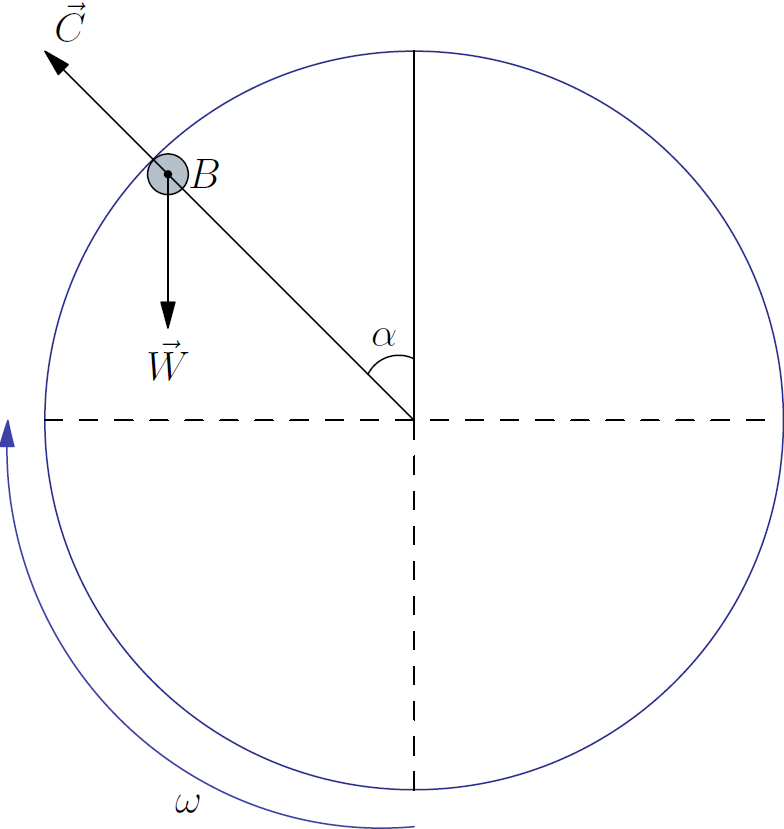
\includegraphics[width=0.5\textwidth]{Images/Preprocesamiento/DBola.PNG}
\caption{Dynamic of a ball.}
\label{DBall}
\end{figure}

Sum of forces in the radial direction gives:

\begin{equation}
\begin{array}{c}
        \sum F_r = 0 = C - W cos \, \alpha \\
        \rightarrow \boxed{C = W cos \, \alpha}
        \label{Fr}
\end{array}
\end{equation}

The dynamic of the ball is defined by:

\begin{equation}
        \vec{C} = m \vec{a_p} 
        \label{dinB}
\end{equation}

Where: $m$ is the mass of the ball and $\vec{a_p}$ is the acceleration vector. The absolute acceleration is equivalent to the sum of three accelerations: rotational acceleration, relative acceleration and the Coriolis acceleration.

\begin{equation}
        \vec{a_p} = \dot{\vec{\omega}} \times \vec{r} + \vec{\omega} \times \left(\vec{\omega} \times \vec{r} \right) + 2 \vec{\omega} \times \left(\dot{\vec{r}} \right) _{rot} + \left(\ddot{\vec{r}} \right) _{f}
        \label{apG}
\end{equation}

The rotational speed of the mill is constant, which implies that the acceleration of the particle behaves as shown on Equation \ref{ap}.

\begin{equation}
        \vec{a_p} = \vec{\omega} \times \left(\vec{\omega} \times \vec{r} \right)
        \tag{6}
        \label{ap}
\end{equation}

Relating Equations \ref{Fr}, \ref{dinB} and \ref{ap}:

\begin{equation}
\begin{array}{c}
        C = W cos \, \alpha = m \left(\omega ^2 r \right) = \left(\frac{W}{g} \right) \left[ \left(\frac{V}{r} \right) ^2 r \right]  \rightarrow \\
        W cos \, \alpha = \frac{W \left(2\pi r N(\alpha) \right)^2}{rg} \rightarrow \boxed{N(\alpha) = \sqrt{\frac{g cos \, \alpha}{4 \pi ^2 r}}}
        \tag{7}
        \label{Nalpha}
\end{array}
\end{equation}

Comparing Equation \ref{Nalpha} with Figure 2, it can be seen that the maximum value of the velocity that the mill should rotate is reached when $\alpha = 0$.

\begin{equation}
        N_{max} = \sqrt{\frac{g}{4 \pi ^2 r}}
        \tag{8}
        \label{N}
\end{equation}

Replacing data shown on Tables \ref{req} and \ref{spec} on Equation \ref{N}, the critical rotational speed $N_{max}$ is of $0.838[rev/s] \rightarrow 50.298[rpm]$. So, the rotational speed $N$ of the mill is $40.24[rpm]$.

\subsection{Number of balls}

The user can specify the diameter of the balls, and how many types there shloud be. The number of balls is calculated by the Equation \ref{Nb}. It has, by default, two types of balls: $2 [cm]$ and $4 [cm]$.

\begin{equation}
        N_b = \frac{V_{Tb}/2}{\frac{4}{3}\pi \left(\frac{D_b}{2} \right) ^2}
        \tag{9}
        \label{Nb}
\end{equation}

Replacing the corresponding data on Equation \ref{Nb}, the number of balls per diameter is:

\begin{itemize}
	\item $2.0[cm] \rightarrow 49$
	\item $4.0[cm] \rightarrow 12$
\end{itemize}